\chapter{Planteamiento del problema}\label{sec:chapterI}
\addcontentsline{toc}{chapter}{Planteamiento del problema}

En la asignatura Desarrollo Basado en Agentes los alumnos, organizados en grupos de 4 o 5 alumnos, se conectan a un Laboratorio remoto de la UGR que está siempre disponible para los mismos. La arquitectura del servidor remoto puede apreciarse en la Figura \ref{fig:architecture}.

\begin{figure}[H]
    \centering
    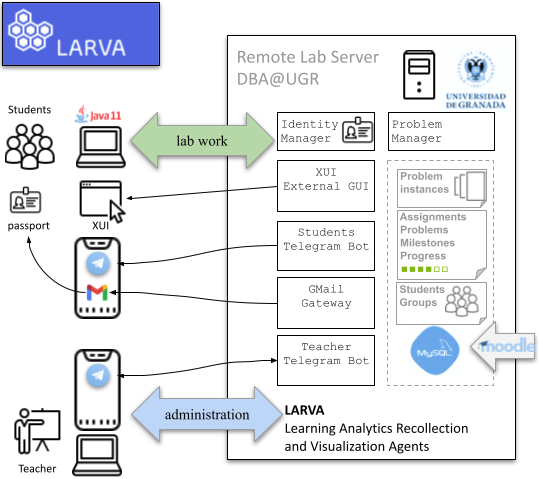
\includegraphics[width=0.60\textwidth]{estado/LARVA2122Architecturec.png}
    \caption{Arquitectura del Servidor Remoto. Por un lado, contiene el laboratorio virtual para sistemas multiagente distribuidos. Además, los alumnos también pueden consultar su progreso y el de sus compañeros a través de un Bot de Telegram en tiempo real. Por otro lado, el profesor también puede conocer el número de objetivos conseguidos por cada uno de sus grupos de alumnos también en tiempo real.}
    \label{fig:architecture}
\end{figure}

Este servidor contiene varios mundos virtuales y se encarga de registrar y almacenar las interacciones con él \cite{Vidal_2016}. Cada mundo virtual es una matriz cuadrada que representa espacios abiertos (en color blanco), obstáculos (en negro) y objetivos (en rojo) tal y como se muestra en la Figura \ref{fig:map}. Los agentes de los alumnos deben entrar en uno de esos mundos virtuales, percibir su vecindario, navegar a través de los espacios abiertos (empleando alguna clase de heurística exploratoria), evitar obstáculos y tratar de llegar al objetivo. En total, cada uno de los problemas planteados requieren de cinco pasos (o \emph{milestones}) hasta su consecución.

\begin{figure}[H]
    \centering
    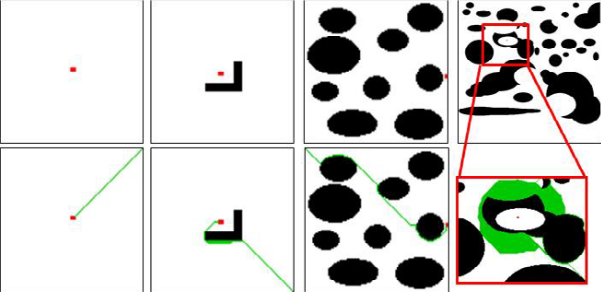
\includegraphics[width=0.60\textwidth]{estado/virtualworlds.png}
    \caption{Alguno de los mapas que el alumnado debe resolver. Los agentes de los grupos de estudiantes deben acceder a uno de esos mundos y deben alcanzar los objetivos (coloreados en rojo) navengado a través del mundo y evitando los obstáculos (coloreados en negro). Alguno de los mundos no son resolubles porque el objetivo no se puede alcanzar con el objetivo de forzar a los agentes de los alumnos a razonar acerca de la irresolubilidad. Las posibles trayectorias están marcadas en verde.}
    \label{fig:map}
\end{figure}

La percepción del agente de su entorno es crítica para resolver estos mundos. En este laboratorio virtual los alumnos pueden configurar cuál de los siguientes sensores estarán enchufados en sus agentes (cualquier combinación de ellos):

\begin{itemize}
	\item Un \textbf{GPS} que indica al agente sus coordenadas $(x,y)$ en el mundo virtual.
	\item Un \textbf{sensor de batería}. Cada agente está alimentado con una batería cuya capacidad es limitada y cuya carga decrece conforme el agente realiza algún movimiento. La batería nunca debe ser vaciada por completo.
	\item Un \textbf{sensor radar} que informa al agente acerca de los tipos de celdas que lo rodean con una percepción local de 5x5 (observar Figura \ref{fig:sensorb}).
	\item Un \textbf{sensor escáner} que actúa como \emph{detector del objetivo} e indica al agente la distancia al mismo medida desde cada una las celdas de su entorno 5x5 (observar Figura \ref{fig:sensorc}).
\end{itemize}

\begin{figure}[H]
\centering
\begin{subfloat}[] {
\centering
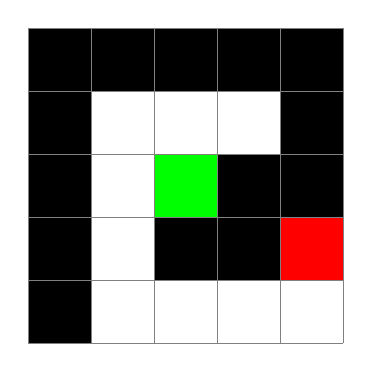
\begin{tikzpicture}[scale=0.8]
	\fill (0,0) rectangle ++ (1,1); 
    \fill (0,1) rectangle ++ (1,1);
    \fill (0,2) rectangle ++ (1,1);
    \fill (0,3) rectangle ++ (1,1);
    \fill (0,4) rectangle ++ (1,1); 
    \fill (1,4) rectangle ++ (1,1);
    \fill (2,4) rectangle ++ (1,1);
    \fill (3,4) rectangle ++ (1,1);
    \fill (4,4) rectangle ++ (1,1);
    \fill (4,3) rectangle ++ (1,1);
    \fill (4,2) rectangle ++ (1,1);
    \fill (3,2) rectangle ++ (1,1);
    \fill (2,1) rectangle ++ (1,1);
    \fill (3,1) rectangle ++ (1,1);
    \fill[red] (4,1) rectangle ++ (1,1);
 	\fill[green] (2,2) rectangle ++ (1,1); 
 	\draw[draw=gray] (0,0) grid (5,5);
\end{tikzpicture}
\label{fig:sensora}   
}
\end{subfloat}   
\hfill  
\begin{subfloat}[] {
\centering
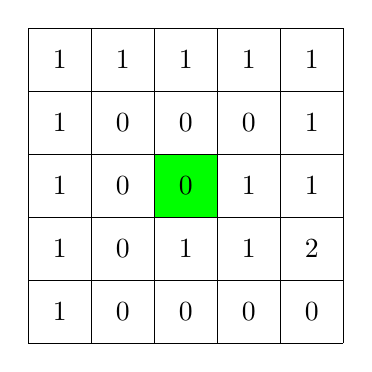
\begin{tikzpicture}[scale=0.8]
\node at (0.5,0.5) {1};
\node at (0.5,1.5) {1};
\node at (0.5,2.5) {1};
\node at (0.5,3.5) {1};
\node at (0.5,4.5) {1};
\node at (1.5,0.5) {0};
\node at (1.5,1.5) {0};
\node at (1.5,2.5) {0};
\node at (1.5,3.5) {0};
\node at (1.5,4.5) {1};
\node at (2.5,0.5) {0};
\node at (2.5,1.5) {1};
\fill[green] (2,2) rectangle ++ (1,1);
\node at (2.5,2.5) {0};
\node at (2.5,3.5) {0};
\node at (2.5,4.5) {1};
\node at (3.5,0.5) {0};
\node at (3.5,1.5) {1};
\node at (3.5,2.5) {1};
\node at (3.5,3.5) {0};
\node at (3.5,4.5) {1};
\node at (4.5,0.5) {0};
\node at (4.5,1.5) {2};
\node at (4.5,2.5) {1};
\node at (4.5,3.5) {1};
\node at (4.5,4.5) {1};
\draw (0,0) grid (5,5);
\end{tikzpicture}
\label{fig:sensorb}   
}    
\end{subfloat}
\hfill
\begin{subfloat}[] {
\centering
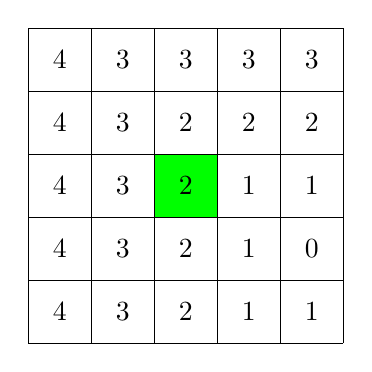
\begin{tikzpicture}[scale=0.8]
\node at (0.5,0.5) {4};
\node at (0.5,1.5) {4};
\node at (0.5,2.5) {4};
\node at (0.5,3.5) {4};
\node at (0.5,4.5) {4};
\node at (1.5,0.5) {3};
\node at (1.5,1.5) {3};
\node at (1.5,2.5) {3};
\node at (1.5,3.5) {3};
\node at (1.5,4.5) {3};
\node at (2.5,0.5) {2};
\node at (2.5,1.5) {2};
\fill[green] (2,2) rectangle ++ (1,1);
\node at (2.5,2.5) {2};
\node at (2.5,3.5) {2};
\node at (2.5,4.5) {3};
\node at (3.5,0.5) {1};
\node at (3.5,1.5) {1};
\node at (3.5,2.5) {1};
\node at (3.5,3.5) {2};
\node at (3.5,4.5) {3};
\node at (4.5,0.5) {1};
\node at (4.5,1.5) {0};
\node at (4.5,2.5) {1};
\node at (4.5,3.5) {2};
\node at (4.5,4.5) {3};
\draw (0,0) grid (5,5);
\end{tikzpicture}
\label{fig:sensorc}
}       
\end{subfloat}
\caption{Un agente (representado por una celda verde en el centro de cada figura) tiene una percepción local de su entorno: solamente percibe el entorno 5x5 de celdas colindantes. El Radar \ref{fig:sensorb} muestra dicho entorno 5x5 que rodea al agente e informa de si una celda está vacía (valor $0$), de si hay un obstáculo (valor $1$) o de si hay un objetivo (valor $2$). El Escáner \ref{fig:sensorc} muestra la distancia de cada una de las celdas colindantes al objetivo.}
\label{fig:sensors}
\end{figure}

Basados en su percepción del mundo virtual, cada agente decidirá ejecutar alguna de las siguientes acciones en su entorno implementando cualquier heurística o proceso de búsqueda.

\begin{itemize}
	\item LOGIN. Entrar en cualquiera de los mundos virtuales.
	\item MOVE. Mover al agente a una de las $8$ celdas adyacentes y gastar una cierta cantidad de batería. Si la celda destino es un obstáculo o el agente se queda sin batería, el agente se rompe y sale del mundo  virtual.
	\item REFUEL. El agente recarga completamente su batería. A los agentes se les permite recargar su batería tantas veces como deseen.
\end{itemize}

\section{Funcionamiento del laboratorio virtual}\label{sec:funcionamiento}

Supongamos que una persona tiene que completar una determinada tarea con nueve pasos o milestones diferentes, numerados del $1$ al $9$, de los cuales los pasos $3$, $6$ y $9$ tienen una recompensa. Esta persona podría intentar pasar por cada una de las subtareas tantas veces como considere oportuno para conseguir todas las recompensas, llevando a cabo un registro de su actividad. Por ejemplo, la Figura \ref{fig:example} muestra uno de estos registros. Ignorando el paso 1, que sólo se utiliza para marcar el inicio del registro, esta persona ha realizado $35$ pasos, repitiendo el paso $2$ siete veces, el paso $3$ seis veces, el paso $4$ dos veces, el paso $5$ seis veces, el paso $6$ cinco veces, el paso $7$ cuatro veces, el paso $8$ cuatro veces y el paso $9$ sólo una vez. Este comportamiento puede representarse con un grafo dirigido ponderado (cíclico) donde los
nodos representan los pasos dados y las aristas se ponderan con la frecuencia detectada en el registro (Figura \ref{fig:example}), de modo que el número de veces que se ejecuta un paso viene dado por la suma de los pesos de sus aristas entrantes, lo cual denominaremos factor de grado de entrada (\emph{in-degree}) de aquí en adelante.

\begin{figure}[H]
    \centering
    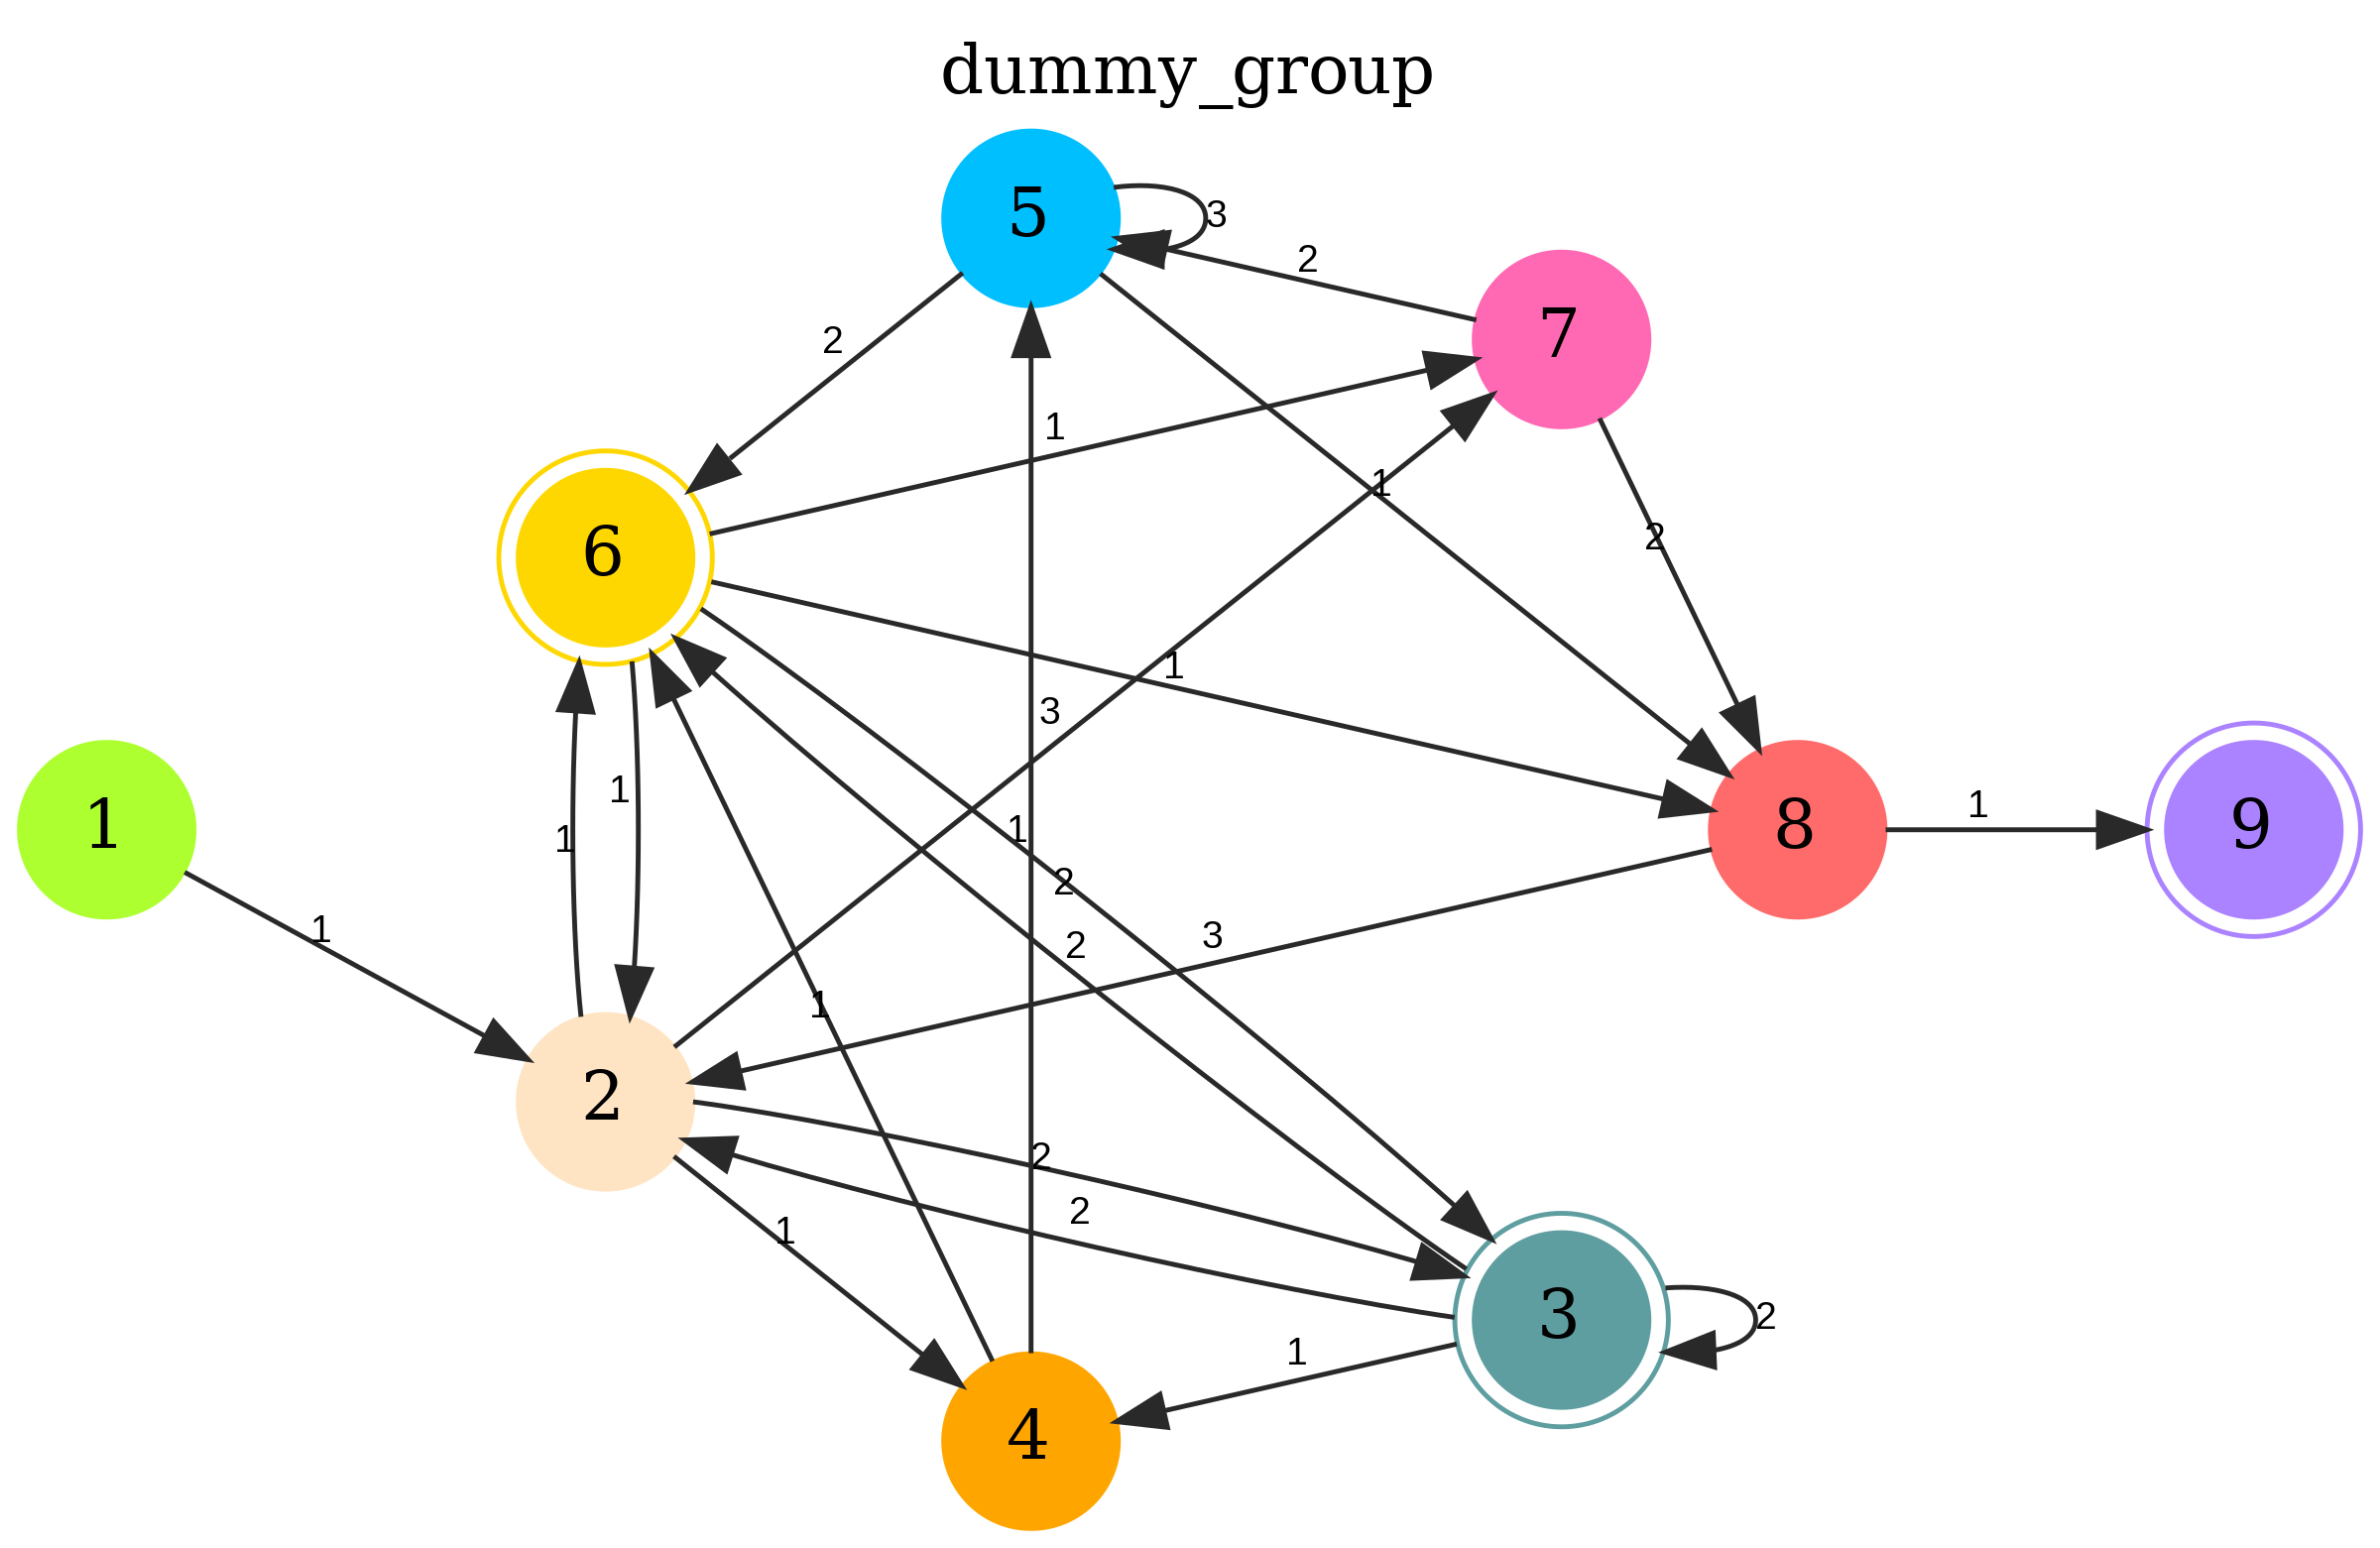
\includegraphics[width=0.60\textwidth]{estado/example.png}
    \caption{La secuencia correspondiente al grafo es: $1$ $2$ $(3)$ $2$ $4$ $5$ $5$ $(6)$ $(3)$ $(3)$ $4$ $(6)$ $7$ $5$ $5$ $5$ $8$ $2$ $(6)$ $(3)$ $2$ $7$ $5$ $(6)$ $8$ $2$ $(3)$ $(3)$ $(6)$ $2$ $7$ $8$ $2$ $7$ $8$ $(9)$. Así pues, el gráfico muestra el comportamiento básico de un determinado grupo en el que se repiten $9$ pasos, tres de los cuales, representados entre paréntesis, tienen una recompensa.}
    \label{fig:example}
\end{figure}

Este registro lineal de actividades refleja exactamente cómo se almacena la realización de tareas de laboratorio en LARVA \cite{Vidal_2022}, \cite{Vidal_2023}, un laboratorio virtual \cite{Vidal_2016} diseñado con un único propósito: permitir a los estudiantes alcanzar su mayor éxito. Para ello, LARVA mantiene un registro completo de la actividad de los alumnos, por lo que su evaluación se basa no sólo en los objetivos alcanzados, sino también en su progreso. Además, cuenta con un sistema de retroalimentación multimodal \cite{Vidal_2022} para mantener a los estudiantes informados sobre su progreso, en tiempo real, gracias a mensajes de chat de Telegram enviados directamente a sus teléfonos móviles. Puede demostrarse que cuanto antes reciban el feedback sobre su actividad y cuanto más rica sea esta retroalimentación, mayor será la autorregulación y la eficacia de la experiencia de aprendizaje \cite{Keller_1968}.

Revelar este comportamiento también puede ser útil para el profesor para detectar, cuanto antes, posibles dificultades de los alumnos para completar sus tareas y permitir una intervención clave por parte del profesor. Pero, ¿cómo detectar estas desviaciones del rendimiento esperado y con qué antelación podrían detectarse? Además, ¿sería posible ignorar cualquier detalle sobre los indicadores de progreso habituales asociados al rendimiento, como el momento de los éxitos y fracasos, la perseverancia, etc., para no depender demasiado en la ``eficiencia clásica'', y centrarse en las características topológicas del comportamiento de los alumnos? En la Figura \ref{fig:extreme} se muestran dos comportamientos extremos. Por un lado, en la Figura \ref{fig:bad}, después de $372$ sesiones, la mayoría de ellas quemadas en los $3$-$4$ primeros objetivos, acaba con muy pocas sesiones en los últimos problemas, una especie de piloto automático, y resuelve $7$ de cada $9$ problemas. Por otro lado, en la Figura \ref{fig:good}, después de $297$ sesiones (¿podría considerarse como un menor esfuerzo?) muestra una exploración bastante exhaustiva de las alternativas y termina con 9 de 9 problemas resueltos. Este
documento responde con éxito a todas estas preguntas a partir de un sólido análisis basado en evidencias de los registros de los últimos siete años de este laboratorio virtual. Las siguientes secciones están dedicadas a discutir trabajos similares en la literatura, a presentar el escenario y la hipótesis principal y, a continuación, a extraer las principales conclusiones tras un análisis exhaustivo de los datos registrados. Todos los conjuntos de datos mencionados en este documento y todos los artefactos de software, completamente escritos en R, están abiertos y disponibles en GitHub \footnote{\href{https://github.com/maribel00/Analysis-of-processes}{https://github.com/maribel00/Analysis-of-processes}}.

\begin{figure}[H]
\centering
\subfloat[Grafo acíclico dirigido que captura el comportamiento de un grupo con $372$ sesiones de trabajo.]{\label{fig:bad}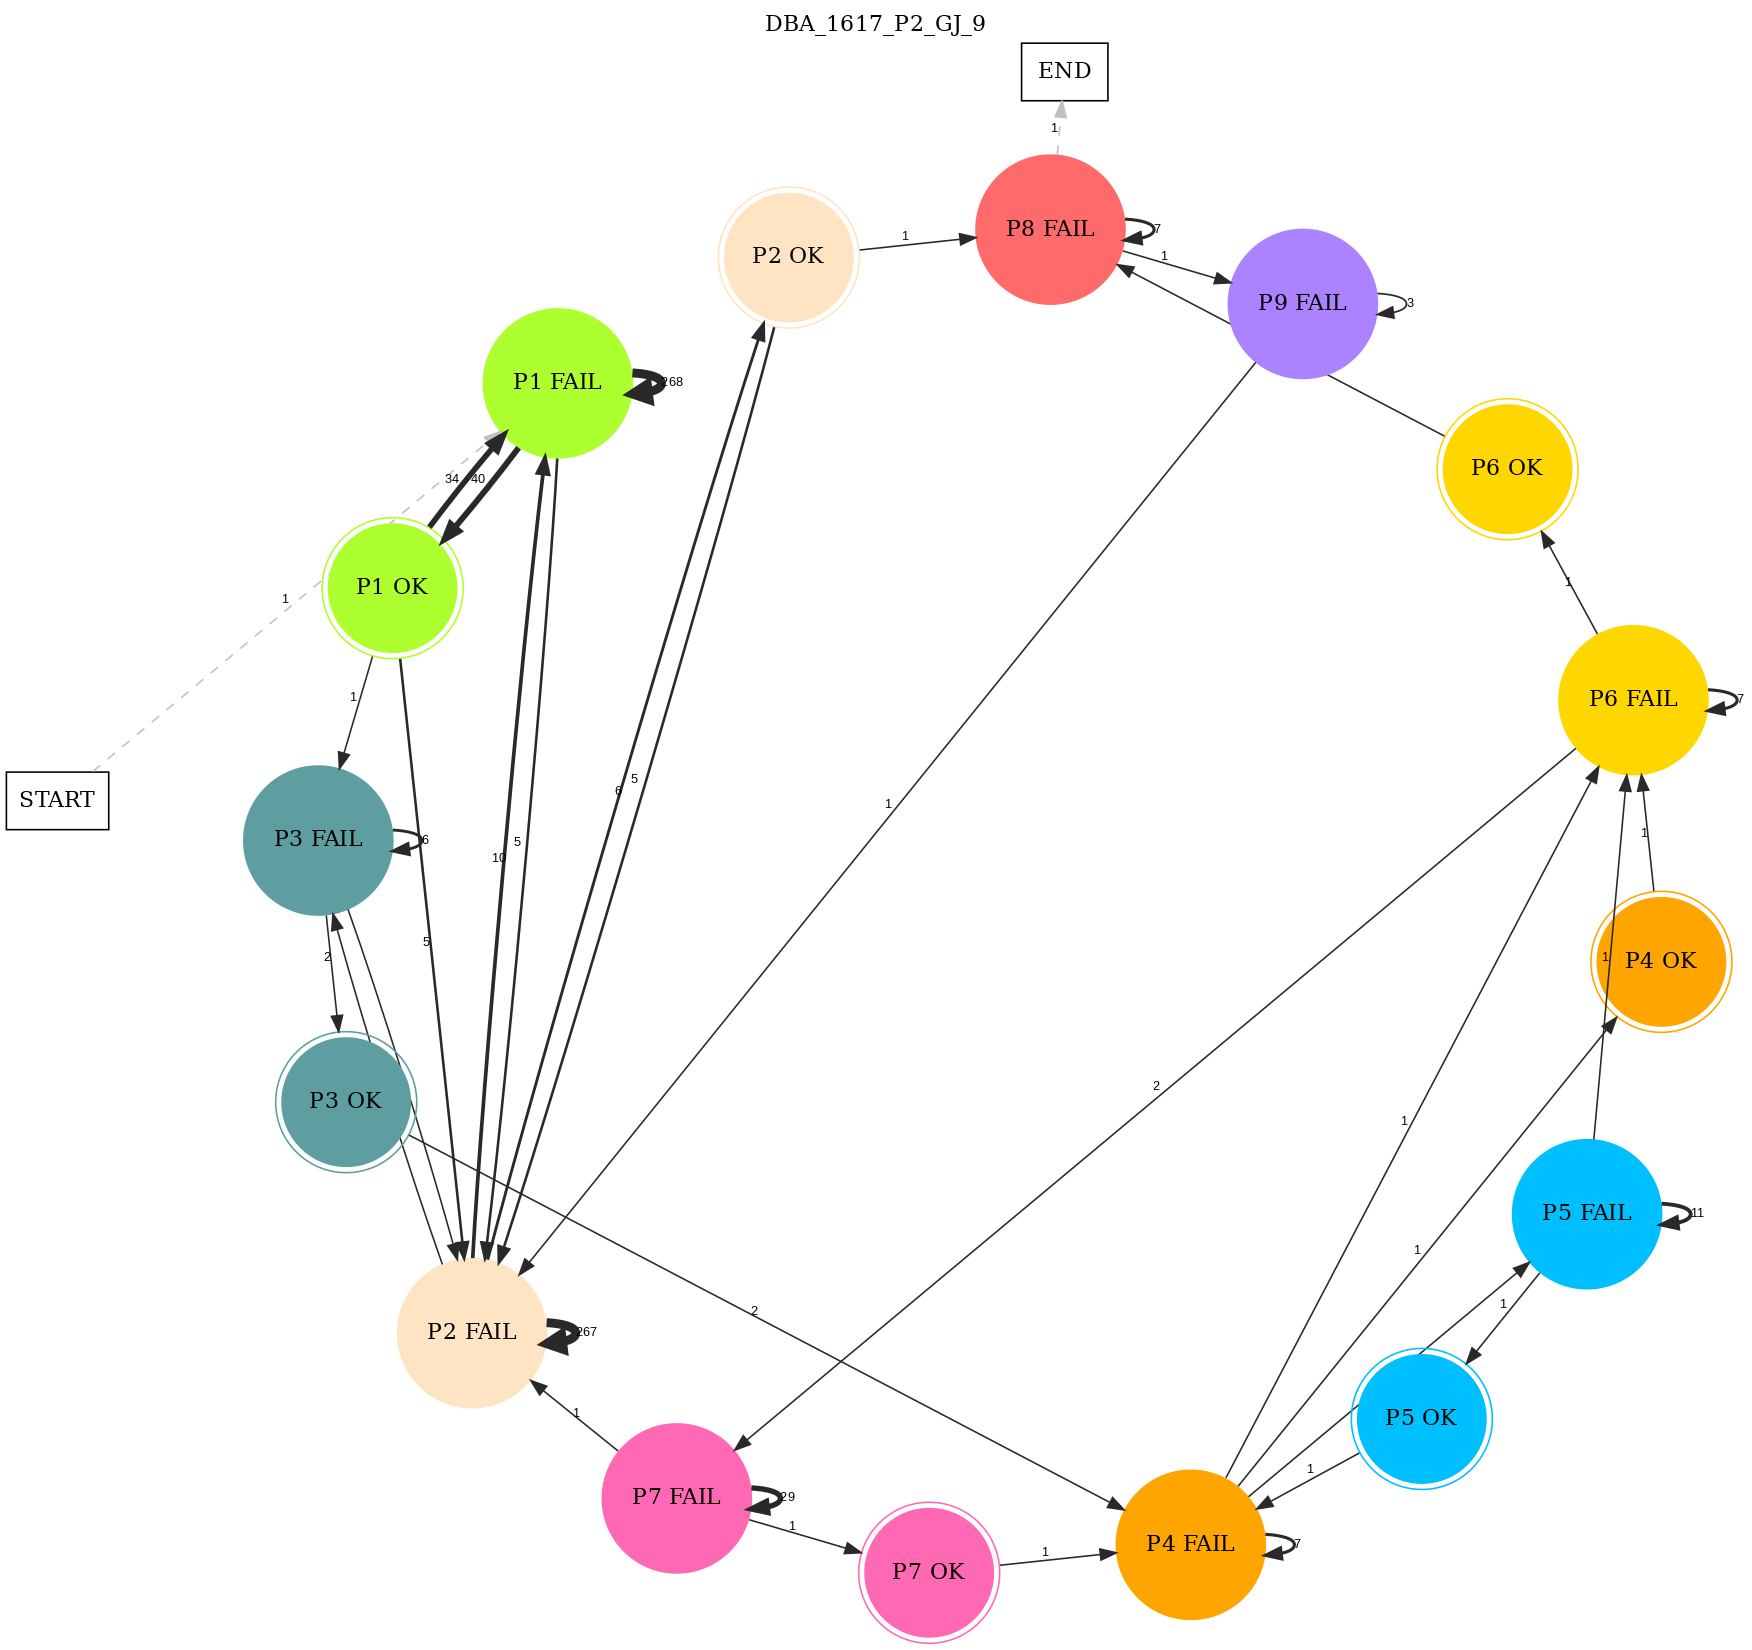
\includegraphics[width=\textwidth]{estado/DBA_1617_P2_GJ_9.png}}\\
\subfloat[Grafo acíclico dirigido que captura el comportamiento de un grupo con $297$ sesiones de trabajo.]{\label{fig:good}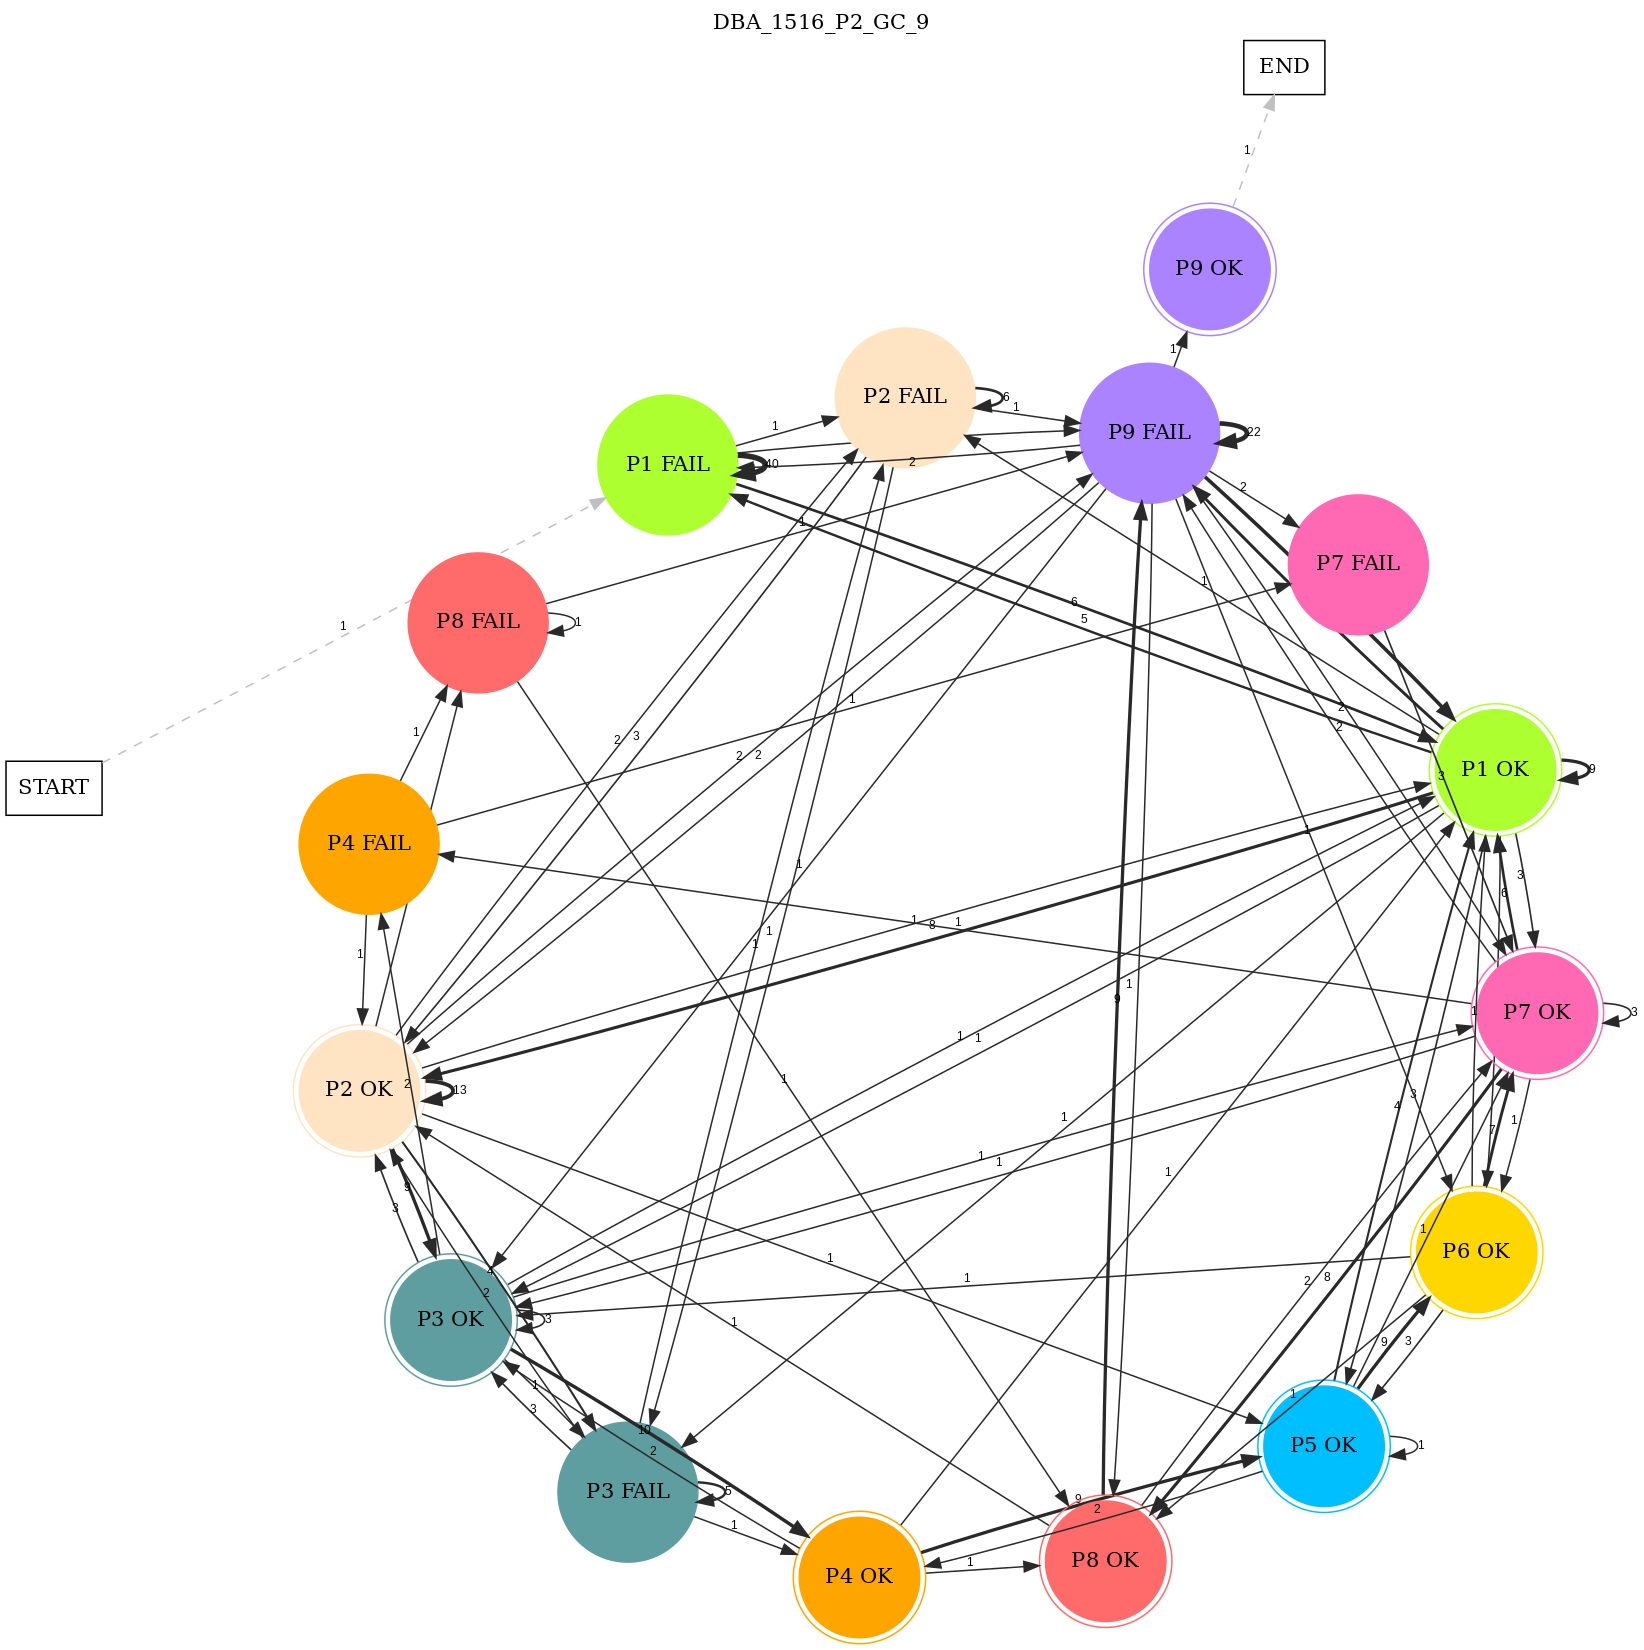
\includegraphics[width=0.6\textwidth]{estado/DBA_1516_P2_GC_9.png}}
\caption{Dos comportamientos reales diferentes de grupos enfrentándose a las mismas tareas de laboratorio.}
\label{fig:extreme}
\end{figure}

\section{Descripción del escenario inicial}\label{sec:initial}

Como se ha mencionado anteriormente, este estudio se ha llevado a cabo a partir de los datos de una asignatura obligataria de 4º curso de la rama Ingeniería del Software en la Universidad de Granada registrados a través de un laboratorio virtual \cite{Vidal_2016}. Esta asignatura sigue la estructura típica del Sistema Personalizado de Instrucción \cite{Keller_1968} donde el progreso de los estudiantes se monitorea continuamente gracias a un sistema de hitos y logros continuos, proporcionando tanta retroalimentación como sea posible y tan pronto como sea posible. Así, durante el curso, los alumnos se organizan en grupos (de $4$-$5$ miembros cada uno) y cada grupo debe resolver una serie de tareas o problemas. De ahora en adelante denotaremos al conjunto de problemas por $P = \left\lbrace p_i \right\rbrace$ y al número de problemas a resolver por $n = |P|$.

Por lo general, el número de problemas es $n = 9$ y podrían considerarse como un conjunto de misiones a realizar en escenarios similares. Adicionalmente, cada problema ha sido cuidadosamente elaborado por el profesor para que requiera un nivel de dificultad creciente por parte de los estudiantes de tal forma que la estrategia para resolver $p_i$ puede no ser lo suficientemente buena resolver $p_{i+1}$ pero la estrategia para resolver $p_{i+1}$ también debe ser válida en $p_i$. Estos problemas están abiertos durante un determinado periodo de tiempo durante el cual los estudiantes pueden abrir los problemas tantas veces como necesiten, ya sea para intentar resolver el problema, para mejorar sus soluciones en estos problemas o para probar nuevas estrategias. Además de esto, cada problema $p_i$ se ha diseñado como una secuencia de $5$ hitos consecutivos, también en nivel creciente de dificultad:

\begin{equation}
p_i = \left\lbrace p_i^1 , p_i^2 , p_i^3 , p_i^4 , p_i^5 \right\rbrace
\end{equation}

siendo $p_i^1$ el suceso de sólo abrir el problema $i$ y $p_i^5$ la obtención de una solución válida para $p_i$. Estos hitos deben ser alcanzados progresivamente por los alumnos, por lo que todo acaba por empujando a los alumnos un poco hacia adelante en sus capacidades \cite{Keller_1968}. Por lo tanto, a medida que los estudiantes progresan en el laboratorio, dejan un registro de sus logros, que se llamará \emph{comportamiento}, $B^g$, de un determinado grupo $g$, y está compuesto por una secuencia de sesiones.

\begin{equation}
B^g = \left\lbrace ^sp_i^k,\dots \right\rbrace
\end{equation}

Cada \emph{sesión} del laboratorio virtual $^sp_i^k$ se etiqueta como el mayor hito $k$ alcanzado en cada problema $p_i$ y un número natural secuencial $s$ que es un registro del tiempo actual del sistema. Además, se utiliza una marca $START$ para señalar el inicio del de laboratorio y un indicador $END$ para señalar el cierre del mismo.

\begin{equation}
B^g = \left\lbrace ^0START \right\rbrace \cup \left\lbrace ^sp_i^k,\dots \right\rbrace \cup \left\lbrace END \right\rbrace
\end{equation}

\begin{table}[H]
\centering
\caption{El comportamiento de un grupo ficticio con $20$ sesiones de trabajo en el laboratorio virtual.}
\label{tab:sequence}
\begin{tabular}{cccccccccccc}
$^0START$ & $^1p_1^1$ & $^2p_1^3$ & $^3p_1^5$ & $^4p_1^5$ & $^5p_1^5$ & $^6p_1^4$ & $^7p_2^3$ & $^8p_2^4$ & $^9p_1^5$ & $^{10}p_1^5$ \\ \hline
$^{11}p_2^5$  & $^{12}p_1^1$ & $^{13}p_2^5$ & $^{14}p_3^2$ & $^{15}p_3^4$ & $^{16}p_1^2$ & $^{17}p_3^3$ & $^{18}p_2^3$ & $^{19}p_3^4$ & $^{20}p_3^5$ & $END$
\end{tabular}
\end{table}

Por ejemplo, en un escenario con tres problemas, la secuencia mostrada en el Cuadro \ref{tab:sequence} podría ser un comportamiento factible $B$, que ya se introdujo en la Sección \ref{sec:funcionamiento}, y ahora se explica bajo una nueva perspectiva:

\emph{``Los estudiantes se han conectado $20$ veces al laboratorio virtual. En la primera sesión se abre el problema $p_1$ sin más éxito y en la segunda sesión se deja el problema $p_1$ a medias. No obstante, en la tercera sesión se resuelve completamente $p_1$ . Los estudiantes ponen en práctica nuevas estrategias y resuelven $p_1$ dos veces más. A continuación, introducen un nuevo cambio que casi resuelve $p_1$, acaba fallando y deja $p_2$ justo en la mitad. Después, tras algunos cambios, resuelven de nuevo $p_1$ en la sesión $9$ y $p_2$ en la sesión $11$. Después, cambiaron algo en la implementación que resultó ser un fracaso en $p_1$ y acaban teniendo éxito en $p_3$ justo al final''.}

La Figura \ref{fig:groupsperyear} y los Cuadros \ref{tab:days} y \ref{tab:records} muestran información descriptiva de los datos registrados cada año sobre el comportamiento de $77$ grupos (en total casi $400$ alumnos). Como se puede ver, hay registros de $7$ años consecutivos y un total de $30672$ sesiones de trabajo en el laboratorio virtual. A continuación, el reto es cómo detectar, lo antes posible, a los grupos con dificultades para progresar.